%%
% This is an Overleaf template for presentations
% using the TUM Corporate Desing https://www.tum.de/cd
%
% For further details on how to use the template, take a look at our
% GitLab repository and browse through our test documents
% https://gitlab.lrz.de/latex4ei/tum-templates.
%
% The tumbeamer class is based on the beamer class.
% If you need further customization please consult the beamer class guide
% https://ctan.org/pkg/beamer.
% Additional class options are passed down to the base class.
%
% If you encounter any bugs or undesired behaviour, please raise an issue
% in our GitLab repository
% https://gitlab.lrz.de/latex4ei/tum-templates/issues
% and provide a description and minimal working example of your problem.
%%

\documentclass{setbeamer}

\usepackage{tikz}
\usepackage{marvosym}
\usetikzlibrary{positioning,graphs,trees,matrix}
\usetikzlibrary{overlay-beamer-styles} % adds [visible on] option for tikz nodes
\usetikzlibrary{arrows.meta} % allows for more specification on how arrows look

\tikzset{
    >=Stealth[round],
    commit/.style = {draw, circle, minimum size = 7mm},
}

\newenvironment{mydirtree}[1][]{
    \begin{tikzpicture}[
        grow via three points = {one child at (0.3,-0.7) and two children at (0.3,-0.7) and (0.3,-1.3)},
        edge from parent path = {(\tikzparentnode.south) circle |- (\tikzchildnode.west)},
        every node/.style = {anchor=west},
        #1
    ]
}{
    \end{tikzpicture}
}


\TUMbeamersetup{
    section page = TUM toc,   % style of section pages
}

% presentation metadata
\title{Version Control}
\subtitle{Git}

\institute{\theChairName\\\theDepartmentName\\\theUniversityName}
\date[05.10.2023]{5. Oktober 2023}

\footline{\insertauthor~|~\insertshorttitle~|~\insertshortdate}

\begin{document}

\maketitle

\begin{frame}{Version Control System}{3 Primärziele}
    \begin{enumerate}
        \item Zugreifen auf frühere Versionen des Quellcodes
        \item Gleichzeitiges Arbeiten an verschiedenen features
        \item Synchronisation mehrer Entwickler
    \end{enumerate}
\end{frame}

% \section{Was ist Git}

% \begin{frame}{Git Historie}
% \end{frame}

\section{Zugreifen auf frühere Versionen des Quellcodes}

\begin{frame}<handout:8,10>[fragile]{Naiver Ansatz}
    Wiederholtes speichern des Projekts bei jeder Änderung.

    \begin{Center}
        \begin{onlyenv}<all:1-8>
            \begin{mydirtree}
                \node (root) {myproject}
                    child [visible on=<2->] { node {V1} }
                    child [visible on=<3->] { node {V2} }
                    child [visible on=<4->] { node {V3} }
                    child [visible on=<5->] { node {VFinal} }
                    child [visible on=<6->] { node {VFinal2} }
                    child [visible on=<7->] { node {VFinalFinal} }
                    child [visible on=<8->] { node {VFinalFinal2} };
            \end{mydirtree}
        \end{onlyenv}

        \begin{onlyenv}<all:9->
            \begin{mydirtree}
                \node (root) {myproject}
                    child { node {V1}
                        child { node {main.c} }
                    }
                    child [missing] {}
                    child { node {V2}
                        child { node {main.c} }
                        child { node {foo.c} }
                    }
                    child [missing] {}
                    child [missing] {}
                    child { node {V3}
                        child { node {main.c} }
                        child { node {bar.c} }
                    };
            \end{mydirtree}
        \end{onlyenv}
    \end{Center}

    \onslide<all:10->{Problem: hohe Redundanz und daher großer Speicheraufwand}
\end{frame}

\begin{frame}[fragile]{Git Commits}
    Idee: Statt immer das ganze Projekt zu speichern, speichert man nur die Änderungen.

    \vspace{3mm}
    \begin{onlyenv}<2->
        \begin{Center}
            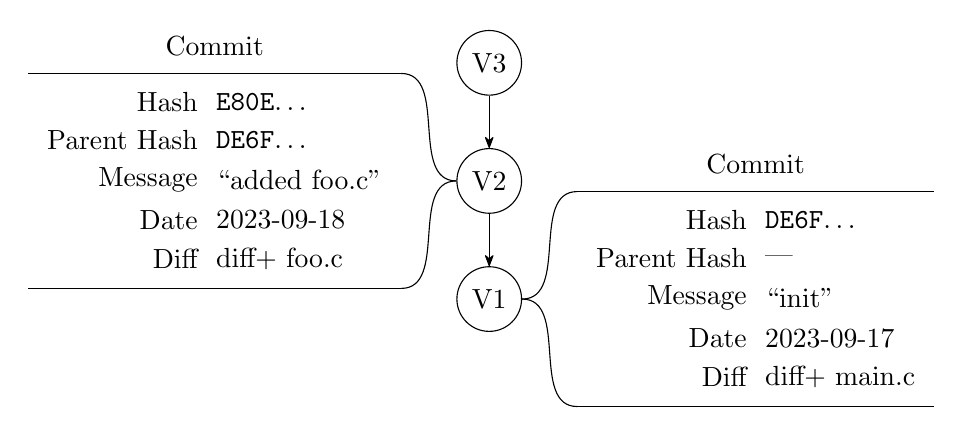
\begin{tikzpicture}
                \graph [grow up = 1.5cm,
                    nodes = {draw, circle, minimum size = 5mm}] { V1 <- V2 <- V3 };

                \onslide<3->
                \matrix (data_a) [right=7mm of V1, matrix of nodes,
                    column 1/.style={anchor=east},
                    column 2/.style={anchor=west},
                ] {
                    Hash & \verb|DE6F|\dots \\
                    Parent Hash & --- \\
                    Message & ``init'' \\
                    Date & 2023-09-17 \\
                    Diff & \mintinline{diff}{+ main.c} \\
                };

                \node [above = 1mm of data_a] {Commit};

                \draw (V1.east) to[out=0, in=180] (data_a.north west);
                \draw (V1.east) to[out=0, in=180] (data_a.south west);
                \draw (data_a.north west) -- (data_a.north east);
                \draw (data_a.south west) -- (data_a.south east);

                \onslide<4->
                \matrix (data_b) [left=7mm of V2, matrix of nodes,
                    column 1/.style={anchor=east},
                    column 2/.style={anchor=west}
                ] {
                    Hash & \verb|E80E|\dots \\
                    Parent Hash & \verb|DE6F|\dots \\
                    Message & ``added foo.c'' \\
                    Date & 2023-09-18 \\
                    Diff & \mintinline{diff}{+ foo.c} \\
                };

                \node [above = 1mm of data_b] {Commit};

                \draw (V2.west) to[out=180, in=0] (data_b.north east);
                \draw (V2.west) to[out=180, in=0] (data_b.south east);
                \draw (data_b.north west) -- (data_b.north east);
                \draw (data_b.south west) -- (data_b.south east);

                \onslide<1->
            \end{tikzpicture}
        \end{Center}
    \end{onlyenv}
\end{frame}

\begin{frame}[c]{Commit Interpretation}{Diff vs. Snapshot}
    \begin{columns}[T]
        \begin{column}{0.5\textwidth}
            \textbf{Commit als Diff}\\Technische Interpretation

            \vspace{3mm}
            Ein Commit speichert nur die Änderungen zum Parent Commit.
        \end{column}

        \begin{column}{0.5\textwidth}
            \textbf{Commit als Snapshot}\\Praktische Interpretation

            \vspace{3mm}
            Ein Commit ist ein Snapshot des Projekts.
        \end{column}
    \end{columns}
\end{frame}

\begin{frame}<handout:1-3>[fragile,c]{HEAD und Working Tree}
    \begin{columns}
        \begin{column}{0.5\textwidth}
            \textbf{Working Tree:}

            \begin{onlyenv}<all:1>
                \begin{Center}
                    \begin{mydirtree}
                        \node (root) {myproject}
                            child { node {main.c} };
                    \end{mydirtree}
                \end{Center}
            \end{onlyenv}

            \begin{onlyenv}<all:2,4>
                \begin{Center}
                    \begin{mydirtree}
                        \node (root) {myproject}
                            child { node {main.c} }
                            child { node {foo.c} };
                    \end{mydirtree}
                \end{Center}
                \begin{TUMCodeBlock}{}{sh}
                    $ git checkout E80E...
                \end{TUMCodeBlock}
            \end{onlyenv}

            \begin{onlyenv}<all:3>
                \begin{Center}
                    \begin{mydirtree}
                        \node (root) {myproject}
                            child { node {main.c} }
                            child { node {bar.c} };
                    \end{mydirtree}
                \end{Center}
                \begin{TUMCodeBlock}{}{sh}
                    $ git checkout 2453...
                \end{TUMCodeBlock}
            \end{onlyenv}
        \end{column}

        \begin{column}{0.5\textwidth}
            \textbf{Commit History:}

            \begin{onlyenv}<all:1>
                \begin{Center}
                    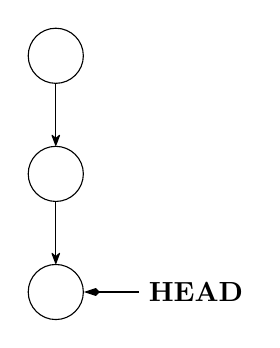
\begin{tikzpicture}
                        \graph [grow up = 1.5cm,
                            nodes = {commit, empty nodes}] { V1 <- V2 <- V3 };

                        \node (head) [right = 7mm of V1] {\textbf{HEAD}};

                        \draw [-Kite] (head.west) -- (V1.east);
                    \end{tikzpicture}
                \end{Center}
            \end{onlyenv}

            \begin{onlyenv}<all:2,4>
                \begin{Center}
                    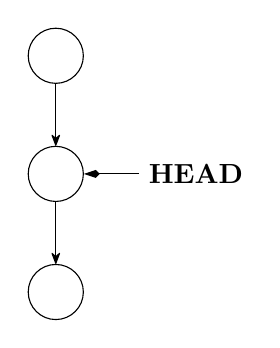
\begin{tikzpicture}
                        \graph [grow up = 1.5cm,
                            nodes = {commit, empty nodes}] { V1 <- V2 <- V3 };

                        \node (head) [right = 7mm of V2] {\textbf{HEAD}};

                        \draw [-Kite] (head.west) -- (V2.east);
                    \end{tikzpicture}
                \end{Center}
            \end{onlyenv}

            \begin{onlyenv}<all:3>
                \begin{Center}
                    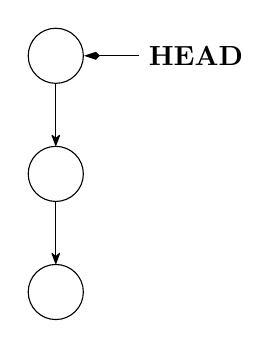
\begin{tikzpicture}
                        \graph [grow up = 1.5cm,
                            nodes = {commit, empty nodes}] { V1 <- V2 <- V3 };

                        \node (head) [right = 7mm of V3] {\textbf{HEAD}};

                        \draw [-Kite] (head.west) -- (V3.east);
                    \end{tikzpicture}
                \end{Center}
            \end{onlyenv}
        \end{column}
    \end{columns}
\end{frame}

\begin{frame}[fragile,t]{Git Repository}
    \begin{columns}[c]
        \begin{column}{0.5\textwidth}
            \begin{Center}
                \begin{mydirtree}[baseline=(root.base)]
                    \node (root) {myproject}
                        child [visible on=<2->] { node {.git} }
                        child { node {main.c} }
                        child { node {bar.c} };
                \end{mydirtree}
            \end{Center}
        \end{column}

        \begin{column}{0.5\textwidth}
            \visible<2->{\TUMCodeInline{text}{git init}}
        \end{column}
    \end{columns}

    \onslide<3->
    \vspace{3mm}
    Der \verb|.git| Ordner speichert alle Informationen die Git braucht, unter anderem:
    \begin{itemize}
        \item Commmits
        \item HEAD
        \item Branches
        \item Remotes
    \end{itemize}

    \vspace{3mm}
    Der Ordner wird von Git verwendet, man sollte ihn also nicht bearbeiten.
\end{frame}

\begin{frame}<handout:2,4,5,8>[fragile]{Erstellen von Commits}{Staging}
    Beim erstellen eines Commits gibt es 3 Stufen:
    \begin{itemize}
        \item Änderungen werden im Working Tree gemacht
        \item Änderungen werden ``gestaged'': \TUMCodeInline{text}{git add <FILES>}
        \item Änderungen werden commited: \TUMCodeInline{text}{git commit -m "<MESSAGE>"}
    \end{itemize}

    \begin{columns}
        \begin{column}{0.25\textwidth}
            \begin{Center}
                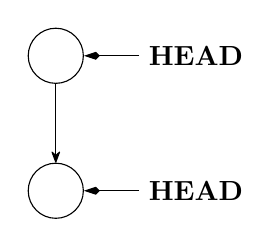
\begin{tikzpicture}
                    \node (V1) [commit] {};

                    \visible<all:5,7->{ \node (V2) [commit, above = 1cm of V1] {}; }
                    \visible<all:5,7->{ \draw[<-] (V1.north) -- (V2.south); }

                    \visible<all:1-4,6>{ \node (head1) [right = 7mm of V1] {\textbf{HEAD}}; }
                    \visible<all:1-4,6>{ \draw [-Kite] (head1.west) -- (V1.east); }

                    \visible<all:5,7->{ \node (head2) [right = 7mm of V2] {\textbf{HEAD}}; }
                    \visible<all:5,7->{ \draw [-Kite] (head2.west) -- (V2.east); }
                \end{tikzpicture}
            \end{Center}
        \end{column}

        \begin{column}{0.25\textwidth}
            \begin{Center}
                \begin{mydirtree}
                    \node (root) {myproject}
                        child { node {main.c} }
                        child [visible on=<all:2->] {
                            node {\only<all:2,3,6->{\textcolor{ForestGreen}{foo.c}}\only<all:4>{\textcolor{orange}{foo.c}}\only<all:5>{foo.c}}
                        };
                \end{mydirtree}
            \end{Center}
        \end{column}

        \begin{column}{0.5\textwidth}
            \begin{onlyenv}<all:1-5>
                \begin{TUMCodeBlock}[minted options={escapeinside=||,beameroverlays=true}]{}{text}
                    |\onslide<all:3-5>|$ git status
                    Untracked files:
                      (use "git add <file>...")
                            foo.c
                    |\onslide<all:4-5>|$ git add foo.c
                    |\onslide<all:5>|$ git commit -m "add foo.c"|\onslide<all:1->|
                \end{TUMCodeBlock}
            \end{onlyenv}

            \begin{onlyenv}<all:6->
                \begin{TUMCodeBlock}[minted options={escapeinside=||,beameroverlays=true}]{}{text}
                    |\onslide<all:7->|$ git commit -m "nothing"
                    |\onslide<all:8->|$ git status
                    Untracked files:
                      (use "git add <file>...")
                            foo.c|\onslide<all:1->|
                \end{TUMCodeBlock}
            \end{onlyenv}
        \end{column}
    \end{columns}

\end{frame}

\section{Gleichzeitiges Arbeiten an verschiedenen features}

\begin{frame}<handout:8,10,11,12,13,14>[fragile,c]{Git Branch}
    \begin{columns}[c]
        \begin{column}{0.5\textwidth}
            \begin{Center}
                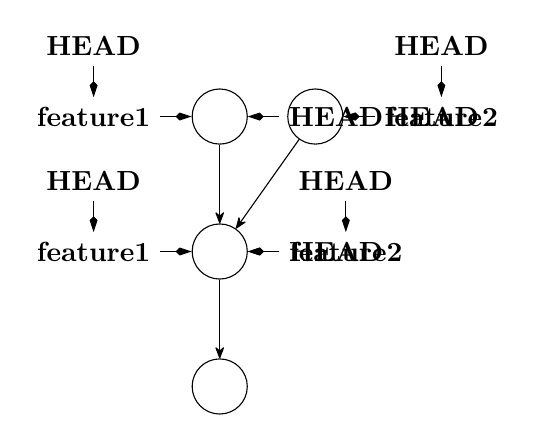
\begin{tikzpicture}
                    % if anyone in the future ever takes over these slides and comes across this
                    % I am so sorry
                    \node (V1) [commit] {};

                    \node (V2) [commit, above = 1cm of V1] {};
                    \draw [<-] (V1) -- (V2);

                    \visible<all:2-4,7,11->{ \node (V3) [commit, above = 1cm of V2] {}; }
                    \visible<all:2-4,7,11->{ \draw [<-] (V2) -- (V3); }

                    \visible<all:4,14->{ \node (V4) [commit, right = 0.5cm of V3] {}; }
                    \visible<all:4,14->{ \draw [<-] (V2) -- (V4); }

                    \visible<all:1,3,5,6,8,9,12>{ \node (head1) [right = 4mm of V2] {\textbf{HEAD}}; }
                    \visible<all:1,3,5,6,8,9,12>{ \draw [-Kite] (head1) -- (V2); }

                    \visible<all:2,7>{ \node (head2) [right = 4mm of V3] {\textbf{HEAD}}; }
                    \visible<all:2,7>{ \draw [-Kite] (head2) -- (V3); }

                    \visible<all:4>{ \node (head3) [right = 4mm of V4] {\textbf{HEAD}}; }
                    \visible<all:4>{ \draw [-Kite] (head3) -- (V4); }

                    \visible<all:6,7,9,10>{ \node (feature1) [left = 4mm of V2] {\textbf{feature1}}; }
                    \visible<all:6,7,9,10>{ \draw [-Kite] (feature1) -- (V2); }
                    \visible<all:10>{ \node (head4) [above = 4mm of feature1] {\textbf{HEAD}}; }
                    \visible<all:10>{ \draw [-Kite] (head4) -- (feature1); }

                    \visible<all:11->{ \node (feature1_2) [left = 4mm of V3] {\textbf{feature1}}; }
                    \visible<all:11->{ \draw [-Kite] (feature1_2) -- (V3); }
                    \visible<all:11>{ \node (head5) [above = 4mm of feature1_2] {\textbf{HEAD}}; }
                    \visible<all:11>{ \draw [-Kite] (head5) -- (feature1_2); }

                    \visible<all:13>{ \node (feature2) [right = 4mm of V2] {\textbf{feature2}}; }
                    \visible<all:13>{ \draw [-Kite] (feature2) -- (V2); }
                    \visible<all:13>{ \node (head6) [above = 4mm of feature2] {\textbf{HEAD}}; }
                    \visible<all:13>{ \draw [-Kite] (head6) -- (feature2); }

                    \visible<all:14->{ \node (feature2_2) [right = 4mm of V4] {\textbf{feature2}}; }
                    \visible<all:14->{ \draw [-Kite] (feature2_2) -- (V4); }
                    \visible<all:14>{ \node (head7) [above = 4mm of feature2_2] {\textbf{HEAD}}; }
                    \visible<all:14>{ \draw [-Kite] (head7) -- (feature2_2); }
                \end{tikzpicture}
            \end{Center}
        \end{column}

        \begin{column}{0.5\textwidth}
            \begin{onlyenv}<all:1-4>
                \begin{TUMCodeBlock}[minted options={escapeinside=||,beameroverlays=true}]{}{text}
                    |\onslide<all:2-4>|$ git commit ...
                    |\onslide<all:3-4>|$ git checkout ...
                    |\onslide<all:4>|$ git commit ...|\onslide<all:1->|
                \end{TUMCodeBlock}
            \end{onlyenv}

            \begin{onlyenv}<all:5,6,7>
                \begin{TUMCodeBlock}[minted options={escapeinside=||,beameroverlays=true}]{}{text}
                    |\onslide<all:6-7>|$ git branch feature1
                    |\onslide<all:7>|$ git commit ...|\onslide<all:1->|
                \end{TUMCodeBlock}
            \end{onlyenv}

            \begin{onlyenv}<all:8->
                \begin{TUMCodeBlock}[minted options={escapeinside=||,beameroverlays=true}]{}{text}
                    |\onslide<all:9->|$ git branch feature1
                    |\onslide<all:10->|$ git checkout feature1
                    |\onslide<all:11->|$ git commit...
                    |\onslide<all:12->|$ git checkout...
                    |\onslide<all:13->|$ git checkout -b feature2
                    |\onslide<all:14->|$ git commit ...|\onslide<all:1->|
                \end{TUMCodeBlock}
            \end{onlyenv}
        \end{column}
    \end{columns}
\end{frame}

\begin{frame}[c]{Detached HEAD}
    Der \textbf{HEAD} Pointer ist \emph{detached} wenn er nicht an einem Branch hängt.

    \begin{TUMBoxFill}[orange]{}{}
        Commits die mit einem \textbf{detached HEAD} erstellt werden, gehen potenziell verloren!
    \end{TUMBoxFill}
\end{frame}

\begin{frame}[c]{Branch Interpretation}{Pointer vs. Subtree}
    \begin{columns}[T]
        \begin{column}{0.5\textwidth}
            \textbf{Branch als Pointer}\\Technische Interpretation

            \vspace{3mm}
            Ein Branch zeigt auf einen einzige Commit.
        \end{column}

        \begin{column}{0.5\textwidth}
            \textbf{Branch als Subtree}\\Praktische Interpretation

            \vspace{3mm}
            Ein Branch ist der komplette Teilbaum aller Vorgänger eines Commits.

            \begin{footnotesize}
                (Alternativ: Alle Vorgänger bis zur ersten Abzweigung.)
            \end{footnotesize}
        \end{column}
    \end{columns}
\end{frame}

\begin{frame}[fragile,c]{Git Merge}{Fast Forward Merge}
    \begin{columns}[c]
        \begin{column}{0.5\textwidth}
            \begin{Center}
                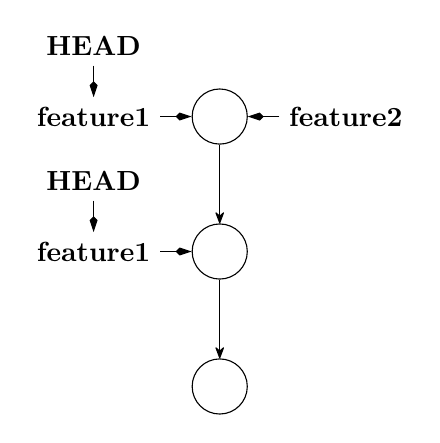
\begin{tikzpicture}
                    \node (V1) [commit] {};

                    \node (V2) [commit, above = 1cm of V1] {};
                    \draw [<-] (V1) -- (V2);

                    \node (V3) [commit, above = 1cm of V2] {};
                    \draw [<-] (V2) -- (V3);

                    \visible<all:1>{ \node (feature1) [left = 4mm of V2] {\textbf{feature1}}; }
                    \visible<all:1>{ \draw [-Kite] (feature1) -- (V2); }
                    \visible<all:1>{ \node (head1) [above = 4mm of feature1] {\textbf{HEAD}}; }
                    \visible<all:1>{ \draw [-Kite] (head1) -- (feature1); }

                    \node (feature2) [right = 4mm of V3] {\textbf{feature2}};
                    \draw [-Kite] (feature2) -- (V3);

                    \visible<all:2->{ \node (feature1_2) [left = 4mm of V3] {\textbf{feature1}}; }
                    \visible<all:2->{ \draw [-Kite] (feature1_2) -- (V3); }
                    \visible<all:2->{ \node (head2) [above = 4mm of feature1_2] {\textbf{HEAD}}; }
                    \visible<all:2->{ \draw [-Kite] (head2) -- (feature1_2); }
                \end{tikzpicture}
            \end{Center}
        \end{column}

        \begin{column}{0.5\textwidth}
            \begin{TUMCodeBlock}[minted options={escapeinside=||,beameroverlays=true}]{}{text}
                |\onslide<all:2->|$ git merge feature2|\onslide<all:1->|
            \end{TUMCodeBlock}
        \end{column}
    \end{columns}
\end{frame}

\begin{frame}[fragile,c]{Git Merge}
    \begin{columns}[c]
        \begin{column}{0.5\textwidth}
            \begin{Center}
                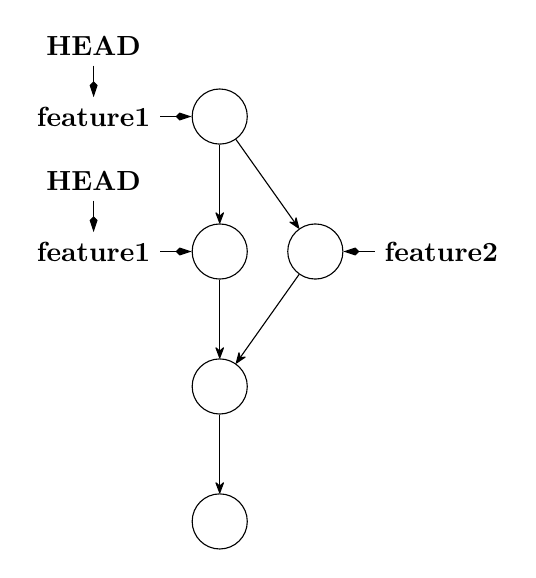
\begin{tikzpicture}
                    \node (V1) [commit] {};

                    \node (V2) [commit, above = 1cm of V1] {};
                    \draw [<-] (V1) -- (V2);

                    \node (V3) [commit, above = 1cm of V2] {};
                    \draw [<-] (V2) -- (V3);

                    \node (V4) [commit, right = 0.5cm of V3] {};
                    \draw [<-] (V2) -- (V4);

                    \visible<all:2->{ \node (V5) [commit, above = 1cm of V3] {}; }
                    \visible<all:2->{ \draw [<-] (V3) -- (V5); }
                    \visible<all:2->{ \draw [<-] (V4) -- (V5); }

                    \visible<all:1>{ \node (feature1) [left = 4mm of V3] {\textbf{feature1}}; }
                    \visible<all:1>{ \draw [-Kite] (feature1) -- (V3); }
                    \visible<all:1>{ \node (head1) [above = 4mm of feature1] {\textbf{HEAD}}; }
                    \visible<all:1>{ \draw [-Kite] (head1) -- (feature1); }

                    \node (feature2) [right = 4mm of V4] {\textbf{feature2}};
                    \draw [-Kite] (feature2) -- (V4);

                    \visible<all:2->{ \node (feature1_2) [left = 4mm of V5] {\textbf{feature1}}; }
                    \visible<all:2->{ \draw [-Kite] (feature1_2) -- (V5); }
                    \visible<all:2->{ \node (head2) [above = 4mm of feature1_2] {\textbf{HEAD}}; }
                    \visible<all:2->{ \draw [-Kite] (head2) -- (feature1_2); }
                \end{tikzpicture}
            \end{Center}
        \end{column}

        \begin{column}{0.5\textwidth}
            \begin{TUMCodeBlock}[minted options={escapeinside=||,beameroverlays=true}]{}{text}
                |\onslide<all:2->|$ git merge feature2|\onslide<all:1->|
            \end{TUMCodeBlock}
        \end{column}
    \end{columns}
\end{frame}

\section{Synchronisation mehrer Entwickler}

\begin{frame}<handout:1,3>[fragile,c]{Git Remotes}
    \begin{columns}[c]
        \begin{column}{0.5\textwidth}
            \begin{Center}
                \begin{figure}
                    \begin{tikzpicture}
                        \node (local) [draw] {
                            \begin{tikzpicture}
                                \visible<all:2->{ \node (V1) [commit] {}; }

                                \visible<all:2->{ \node (V2) [commit, above = 1cm of V1] {}; }
                                \visible<all:2->{ \draw [<-] (V1) -- (V2); }

                                \visible<all:2->{ \node (master) [below left = -2mm and 5mm of V2] {\textbf{master}}; }
                                \visible<all:2->{ \draw [-Kite] (master) -- (V2); }

                                \visible<all:2->{ \node (head) [left = 4mm of master] {\textbf{HEAD}}; }
                                \visible<all:2->{ \draw [-Kite] (head) -- (master); }

                                \visible<all:2->{ \node (origin_master) [above left = -2mm and 5mm of V2] {\textbf{origin/master}}; }
                                \visible<all:2->{ \draw [-Kite] (origin_master) -- (V2); }
                            \end{tikzpicture}
                        };
                    \end{tikzpicture}
                    \caption*{local}
                \end{figure}
            \end{Center}
        \end{column}

        \begin{column}{0.5\textwidth}
            \begin{Center}
                \begin{figure}
                    \begin{tikzpicture}
                        \node (remote) [draw] {
                            \begin{tikzpicture}
                                \node (V1) [commit] {};

                                \node (V2) [commit, above = 1cm of V1] {};
                                \draw [<-] (V1) -- (V2);

                                \node (master) [left = 4mm of V2] {\textbf{master}};
                                \draw [-Kite] (master) -- (V2);
                            \end{tikzpicture}
                        };
                    \end{tikzpicture}
                    \caption*{remote}
                \end{figure}
            \end{Center}
        \end{column}
    \end{columns}

    \begin{TUMCodeBlock}[minted options={escapeinside=||,beameroverlays=true}]{}{text}
        |\onslide<all:2->|$ git clone <REMOTE_URL>
        |\onslide<all:3->|$ git remote
        origin|\onslide<all:1->|
    \end{TUMCodeBlock}
\end{frame}

\begin{frame}<handout:1,3>[fragile,c]{Git Fetch}
    \begin{columns}[c]
        \begin{column}{0.5\textwidth}
            \begin{Center}
                \begin{figure}
                    \begin{tikzpicture}
                        \node (local) [draw] {
                            \begin{tikzpicture}
                                \node (V1) [commit] {};

                                \node (V2) [commit, above = 0.7cm of V1] {};
                                \draw [<-] (V1) -- (V2);

                                % initial state
                                \visible<all:1>{ \node (master) [below left = -2mm and 5mm of V2] {\textbf{master}}; }
                                \visible<all:1>{ \draw [-Kite] (master) -- (V2); }

                                \visible<all:1>{ \node (head) [left = 4mm of master] {\textbf{HEAD}}; }
                                \visible<all:1>{ \draw [-Kite] (head) -- (master); }

                                \visible<all:1>{ \node (origin_master) [above left = -2mm and 5mm of V2] {\textbf{origin/master}}; }
                                \visible<all:1>{ \draw [-Kite] (origin_master) -- (V2); }

                                % after fetching
                                \visible<all:2->{ \node (V3) [commit, above = 0.7cm of V2] {}; }
                                \visible<all:2->{ \draw [<-] (V2) -- (V3); }

                                \visible<all:2>{ \node (master2) [left = 4mm of V2] {\textbf{master}}; }
                                \visible<all:2>{ \draw [-Kite] (master2) -- (V2); }

                                \visible<all:2>{ \node (head2) [left = 4mm of master2] {\textbf{HEAD}}; }
                                \visible<all:2>{ \draw [-Kite] (head2) -- (master2); }

                                \visible<all:2>{ \node (origin_master2) [left = 4mm of V3] {\textbf{origin/master}}; }
                                \visible<all:2>{ \draw [-Kite] (origin_master2) -- (V3); }

                                % after merging
                                \visible<all:3->{ \node (master3) [below left = -2mm and 5mm of V3] {\textbf{master}}; }
                                \visible<all:3->{ \draw [-Kite] (master3) -- (V3); }

                                \visible<all:3->{ \node (head3) [left = 4mm of master3] {\textbf{HEAD}}; }
                                \visible<all:3->{ \draw [-Kite] (head3) -- (master3); }

                                \visible<all:3->{ \node (origin_master3) [above left = -2mm and 5mm of V3] {\textbf{origin/master}}; }
                                \visible<all:3->{ \draw [-Kite] (origin_master3) -- (V3); }
                            \end{tikzpicture}
                        };
                    \end{tikzpicture}
                    \caption*{local}
                \end{figure}
            \end{Center}
        \end{column}

        \begin{column}{0.5\textwidth}
            \begin{Center}
                \begin{figure}
                    \begin{tikzpicture}
                        \node (remote) [draw] {
                            \begin{tikzpicture}
                                \node (V1) [commit] {};

                                \node (V2) [commit, above = 0.7cm of V1] {};
                                \draw [<-] (V1) -- (V2);

                                \node (V3) [commit, above = 0.7cm of V2] {};
                                \draw [<-] (V2) -- (V3);

                                \node (master) [left = 4mm of V3] {\textbf{master}};
                                \draw [-Kite] (master) -- (V3);
                            \end{tikzpicture}
                        };
                    \end{tikzpicture}
                    \caption*{remote}
                \end{figure}
            \end{Center}
        \end{column}
    \end{columns}

    \vspace{-2mm}

    \begin{TUMCodeBlock}[minted options={escapeinside=||,beameroverlays=true}]{}{text}
        |\onslide<all:2->|$ git fetch
        |\onslide<all:3->|$ git merge origin/master|\onslide<all:1->|
    \end{TUMCodeBlock}
\end{frame}

\begin{frame}[fragile,c]{Git Pull}
    Die Kombination aus \TUMCodeInline{sh}{git fetch} und \TUMCodeInline{sh}{git merge origin/master} ist so häufig, dass es einen eigenen Command dafür gibt: \TUMCodeInline{sh}{git pull}.

    \tikzset{commit/.style = {draw, circle, minimum size = 6mm}}

    \begin{columns}[c]
        \begin{column}{0.5\textwidth}
            \begin{Center}
                \begin{figure}
                    \begin{tikzpicture}
                        \node (local) [draw] {
                            \begin{tikzpicture}
                                \node (V1) [commit] {};

                                \node (V2) [commit, above = 0.6cm of V1] {};
                                \draw [<-] (V1) -- (V2);

                                % initial state
                                \visible<all:1>{ \node (master) [below left = -2mm and 5mm of V2] {\textbf{master}}; }
                                \visible<all:1>{ \draw [-Kite] (master) -- (V2); }

                                \visible<all:1>{ \node (head) [left = 4mm of master] {\textbf{HEAD}}; }
                                \visible<all:1>{ \draw [-Kite] (head) -- (master); }

                                \visible<all:1>{ \node (origin_master) [above left = -2mm and 5mm of V2] {\textbf{origin/master}}; }
                                \visible<all:1>{ \draw [-Kite] (origin_master) -- (V2); }

                                % after pull
                                \visible<all:2->{ \node (V3) [commit, above = 0.6cm of V2] {}; }
                                \visible<all:2->{ \draw [<-] (V2) -- (V3); }

                                \visible<all:2->{ \node (master3) [below left = -2mm and 5mm of V3] {\textbf{master}}; }
                                \visible<all:2->{ \draw [-Kite] (master3) -- (V3); }

                                \visible<all:2->{ \node (head3) [left = 4mm of master3] {\textbf{HEAD}}; }
                                \visible<all:2->{ \draw [-Kite] (head3) -- (master3); }

                                \visible<all:2->{ \node (origin_master3) [above left = -2mm and 5mm of V3] {\textbf{origin/master}}; }
                                \visible<all:2->{ \draw [-Kite] (origin_master3) -- (V3); }
                            \end{tikzpicture}
                        };
                    \end{tikzpicture}
                    \caption*{local}
                \end{figure}
            \end{Center}
        \end{column}

        \begin{column}{0.5\textwidth}
            \begin{Center}
                \begin{figure}
                    \begin{tikzpicture}
                        \node (remote) [draw] {
                            \begin{tikzpicture}
                                \node (V1) [commit] {};

                                \node (V2) [commit, above = 0.6cm of V1] {};
                                \draw [<-] (V1) -- (V2);

                                \node (V3) [commit, above = 0.6cm of V2] {};
                                \draw [<-] (V2) -- (V3);

                                \node (master) [left = 4mm of V3] {\textbf{master}};
                                \draw [-Kite] (master) -- (V3);
                            \end{tikzpicture}
                        };
                    \end{tikzpicture}
                    \caption*{remote}
                \end{figure}
            \end{Center}
        \end{column}
    \end{columns}

    \vspace{-2mm}

    \begin{TUMCodeBlock}[minted options={escapeinside=||,beameroverlays=true}]{}{text}
        |\onslide<all:2->|$ git pull|\onslide<all:1->|
    \end{TUMCodeBlock}
\end{frame}

\begin{frame}<handout:3,5>[fragile,c]{Git Pull mit Merge Commit}
    \tikzset{commit/.style = {draw, circle, minimum size = 6mm}}

    \begin{columns}[c]
        \begin{column}{0.7\textwidth}
            \begin{Center}
                \begin{figure}
                    \begin{tikzpicture}
                        \node (local) [draw] {
                            \begin{tikzpicture}
                                \node (V1) [commit] {};

                                \node (V2) [commit, above = 0.6cm of V1] {};
                                \draw [<-] (V1) -- (V2);

                                % initial state
                                \visible<all:1>{ \node (master) [left = 4mm of V2] {\textbf{master}}; }
                                \visible<all:1>{ \draw [-Kite] (master) -- (V2); }

                                \visible<all:1>{ \node (head) [left = 4mm of master] {\textbf{HEAD}}; }
                                \visible<all:1>{ \draw [-Kite] (head) -- (master); }

                                \visible<all:1-3>{ \node (origin_master) [right = 4mm of V2] {\textbf{origin/master}}; }
                                \visible<all:1-3>{ \draw [-Kite] (origin_master) -- (V2); }

                                % after commit
                                \visible<all:2->{ \node (V3) [commit, above = 0.6cm of V2] {}; }
                                \visible<all:2->{ \draw [<-] (V2) -- (V3); }

                                \visible<all:2-4>{ \node (master2) [left = 4mm of V3] {\textbf{master}}; }
                                \visible<all:2-4>{ \draw [-Kite] (master2) -- (V3); }

                                \visible<all:2-4>{ \node (head2) [left = 4mm of master2] {\textbf{HEAD}}; }
                                \visible<all:2-4>{ \draw [-Kite] (head2) -- (master2); }

                                % after fetch
                                \visible<all:4->{ \node (V4) [commit, right = 0.3cm of V3] {}; }
                                \visible<all:4->{ \draw [<-] (V2) -- (V4); }

                                \visible<all:4->{ \node (origin_master2) [right = 4mm of V4] {\textbf{origin/master}}; }
                                \visible<all:4->{ \draw [-Kite] (origin_master2) -- (V4); }

                                % after merge
                                \visible<all:5->{ \node (V5) [commit, above = 0.6cm of V3] {}; }
                                \visible<all:5->{ \draw [<-] (V3) -- (V5); }
                                \visible<all:5->{ \draw [<-] (V4) -- (V5); }

                                \visible<all:5->{ \node (master3) [left = 4mm of V5] {\textbf{master}}; }
                                \visible<all:5->{ \draw [-Kite] (master3) -- (V5); }

                                \visible<all:5->{ \node (head3) [left = 4mm of master3] {\textbf{HEAD}}; }
                                \visible<all:5->{ \draw [-Kite] (head3) -- (master3); }
                            \end{tikzpicture}
                        };
                    \end{tikzpicture}
                    \caption*{local}
                \end{figure}
            \end{Center}
        \end{column}

        \begin{column}{0.3\textwidth}
            \begin{Center}
                \begin{figure}
                    \begin{tikzpicture}
                        \node (remote) [draw] {
                            \begin{tikzpicture}
                                \node (V1) [commit] {};

                                \node (V2) [commit, above = 0.6cm of V1] {};
                                \draw [<-] (V1) -- (V2);

                                \visible<all:1-2>{ \node (master) [right = 4mm of V2] {\textbf{master}}; }
                                \visible<all:1-2>{ \draw [-Kite] (master) -- (V2); }

                                \node (V3) [commit, draw = none, above = 0.6cm of V2] {};

                                \visible<all:3->{ \node (V4) [commit, right = 0.3cm of V3] {}; }
                                \visible<all:3->{ \draw [<-] (V2) -- (V4); }

                                \visible<all:3->{ \node (master2) [right = 4mm of V4] {\textbf{master}}; }
                                \visible<all:3->{ \draw [-Kite] (master2) -- (V4); }
                            \end{tikzpicture}
                        };
                    \end{tikzpicture}
                    \caption*{remote}
                \end{figure}
            \end{Center}
        \end{column}
    \end{columns}

    \vspace{-2mm}

    \begin{TUMCodeBlock}[minted options={escapeinside=||,beameroverlays=true}]{}{text}
        |\onslide<all:4->|$ git fetch
        |\onslide<all:5->|$ git merge origin/master|\onslide<all:1->|
    \end{TUMCodeBlock}
\end{frame}

\begin{frame}[fragile,c]{Git Push}
    \begin{columns}[c]
        \begin{column}{0.7\textwidth}
            \begin{Center}
                \begin{figure}
                    \begin{tikzpicture}
                        \node (local) [draw] {
                            \begin{tikzpicture}
                                \node (V1) [commit] {};

                                \node (V2) [commit, above = 0.6cm of V1] {};
                                \draw [<-] (V1) -- (V2);

                                \node (V3) [commit, above = 0.6cm of V2] {};
                                \draw [<-] (V2) -- (V3);

                                % initial state
                                \visible<all:1>{ \node (master) [left = 4mm of V3] {\textbf{master}}; }
                                \visible<all:1>{ \draw [-Kite] (master) -- (V3); }

                                \visible<all:1>{ \node (head) [left = 4mm of master] {\textbf{HEAD}}; }
                                \visible<all:1>{ \draw [-Kite] (head) -- (master); }

                                \visible<all:1>{ \node (origin_master) [left = 4mm of V2] {\textbf{origin/master}}; }
                                \visible<all:1>{ \draw [-Kite] (origin_master) -- (V2); }

                                % after push
                                \visible<all:2->{ \node (master2) [above left = -2mm and 5mm of V3] {\textbf{master}}; }
                                \visible<all:2->{ \draw [-Kite] (master2) -- (V3); }

                                \visible<all:2->{ \node (head2) [left = 4mm of master2] {\textbf{HEAD}}; }
                                \visible<all:2->{ \draw [-Kite] (head2) -- (master2); }

                                \visible<all:2->{ \node (origin_master2) [below left = -2mm and 5mm of V3] {\textbf{origin/master}}; }
                                \visible<all:2->{ \draw [-Kite] (origin_master2) -- (V3); }
                            \end{tikzpicture}
                        };
                    \end{tikzpicture}
                    \caption*{local}
                \end{figure}
            \end{Center}
        \end{column}

        \begin{column}{0.3\textwidth}
            \begin{Center}
                \begin{figure}
                    \begin{tikzpicture}
                        \node (remote) [draw] {
                            \begin{tikzpicture}
                                \node (V1) [commit] {};

                                \node (V2) [commit, above = 0.6cm of V1] {};
                                \draw [<-] (V1) -- (V2);

                                \visible<all:1>{ \node (master) [left = 4mm of V2] {\textbf{master}}; }
                                \visible<all:1>{ \draw [-Kite] (master) -- (V2); }

                                % after push
                                \visible<all:2->{ \node (V3) [commit, above = 0.6cm of V2] {}; }
                                \visible<all:2->{ \draw [<-] (V2) -- (V3); }

                                \visible<all:2->{ \node (master2) [left = 4mm of V3] {\textbf{master}}; }
                                \visible<all:2->{ \draw [-Kite] (master2) -- (V3); }
                            \end{tikzpicture}
                        };
                    \end{tikzpicture}
                    \caption*{remote}
                \end{figure}
            \end{Center}
        \end{column}
    \end{columns}

    \vspace{-2mm}

    \begin{TUMCodeBlock}[minted options={escapeinside=||,beameroverlays=true}]{}{text}
        |\onslide<all:2->|$ git push|\onslide<all:1->|
    \end{TUMCodeBlock}
\end{frame}

\begin{frame}{Empfehlungen zur Verwendung von Git}
    Wenn man mit anderen Entwicklern arbeitet, ist die typische Reihenfolge für Änderungen:

    \begin{Center}
        \TUMCodeInline{sh}{git add} {\Large\MVRightarrow{}} \TUMCodeInline{sh}{git commit} {\Large\MVRightarrow{}} \TUMCodeInline{sh}{git pull} {\Large\MVRightarrow{}} \TUMCodeInline{sh}{git push}
    \end{Center}

    \vspace{3mm}

    Für komplexe Projekte sollte man sich früh für eine Branch-Ideologie entscheiden, z.~B.~\myhref{https://www.atlassian.com/git/tutorials/comparing-workflows/gitflow-workflow}{Git~Flow}.
\end{frame}

\begin{frame}{GitHub und GitLab}
    Für Remote Server kann man entweder einen eigenen Server hosten (mithilfe von z.~B.~\myhref{https://about.gitea.com}{Gitea}), oder einen existierenden Service verwenden, wie \myhref{https://github.com}{GitHub} oder \myhref{https://gitlab.com}{GitLab}.

    \vspace{3mm}

    GitHub:
    \begin{itemize}
        \item 2018 von Microsoft aufgekauft worden
        \item Der bei weitem verbreiteste Service in der Open Source Welt
    \end{itemize}

    \vspace{3mm}

    GitLab:
    \begin{itemize}
        \item Eigenständig und größtenteils Open Source (oder zumindest source-available)
        \item Self-Hosting möglich (z.~B. auch die \myhref{https://gitlab.lrz.de}{LRZ GitLab Instanz})
    \end{itemize}

    \vspace{3mm}

    \begin{TUMBoxFill}[orange]{}{}
        GitHub und GitLab sind \textbf{Services} auf denen man Git Repositories hosten kann, Git selber hat aber nichts mir diesen Services zu tun und kann auch komplett lokal verwendet werden!
    \end{TUMBoxFill}
\end{frame}

\begin{frame}{Git vegisst nichts}
    Die Git History ist an sich \emph{unveränderlich}. Es ist zwar möglich die History zu ändern, aber recht umständlich und eigentlich nicht angedacht. Um Änderungen rückgängig zu machen, würde man einen neuen Commit erstellen, der die Änderungen rückgängig macht.

    \vspace{3mm}

    Spätestens wenn Sie einen Commit pushen, können Sie diesen nicht mehr leicht löschen.

    \pause
    \vspace{3mm}

    \begin{TUMBoxFill}[orange]{}{}
        Committen Sie keine Secrets wie Passwörter!
    \end{TUMBoxFill}

    \pause
    \vspace{3mm}

    \begin{TUMBoxFill}[orange]{}{}
        Wenn Sie große Dateien committen, sind diese Dateien immer noch in voller Größe vorhanden, auch wenn Sie in einem anderen Commit die Datei wieder löschen!
    \end{TUMBoxFill}

    % TODO git is for text
    % TODO git is not a backup
\end{frame}

% TODO add a demo

\begin{frame}{Git Alternativen}
    \begin{TUMBoxInverse}{}{Mercurial}
        In Verwendung von z. B. Facebook, Mozilla, und das VCS vom TUM-Entwickelten Proof Assistant \myhref{https://isabelle.in.tum.de/}{Isabelle}.
    \end{TUMBoxInverse}

    \begin{TUMBoxInverse}{}{Apache Subversion | SVN}
    \end{TUMBoxInverse}

    \begin{TUMBoxInverse}{}{Google Piper}
        Google's internes VCS zum verwalten eines 2\texttt{+} Milliarden Zeilen Code Monorepository.
    \end{TUMBoxInverse}
\end{frame}

\end{document}
